Before we started coding we made a draft of the class diagrams. Throughout the following sprints we kept maintaining and updating the class diagram
draft to make sure that the code and class diagram were in agreement. The class diagram shown and explained below is the final version for our
system.

The class diagram is made in the Unified Modeling Language (UML) to ensure common understanding, when describing the structure of our system.

\begin{figure}[htb]
    \begin{center}
        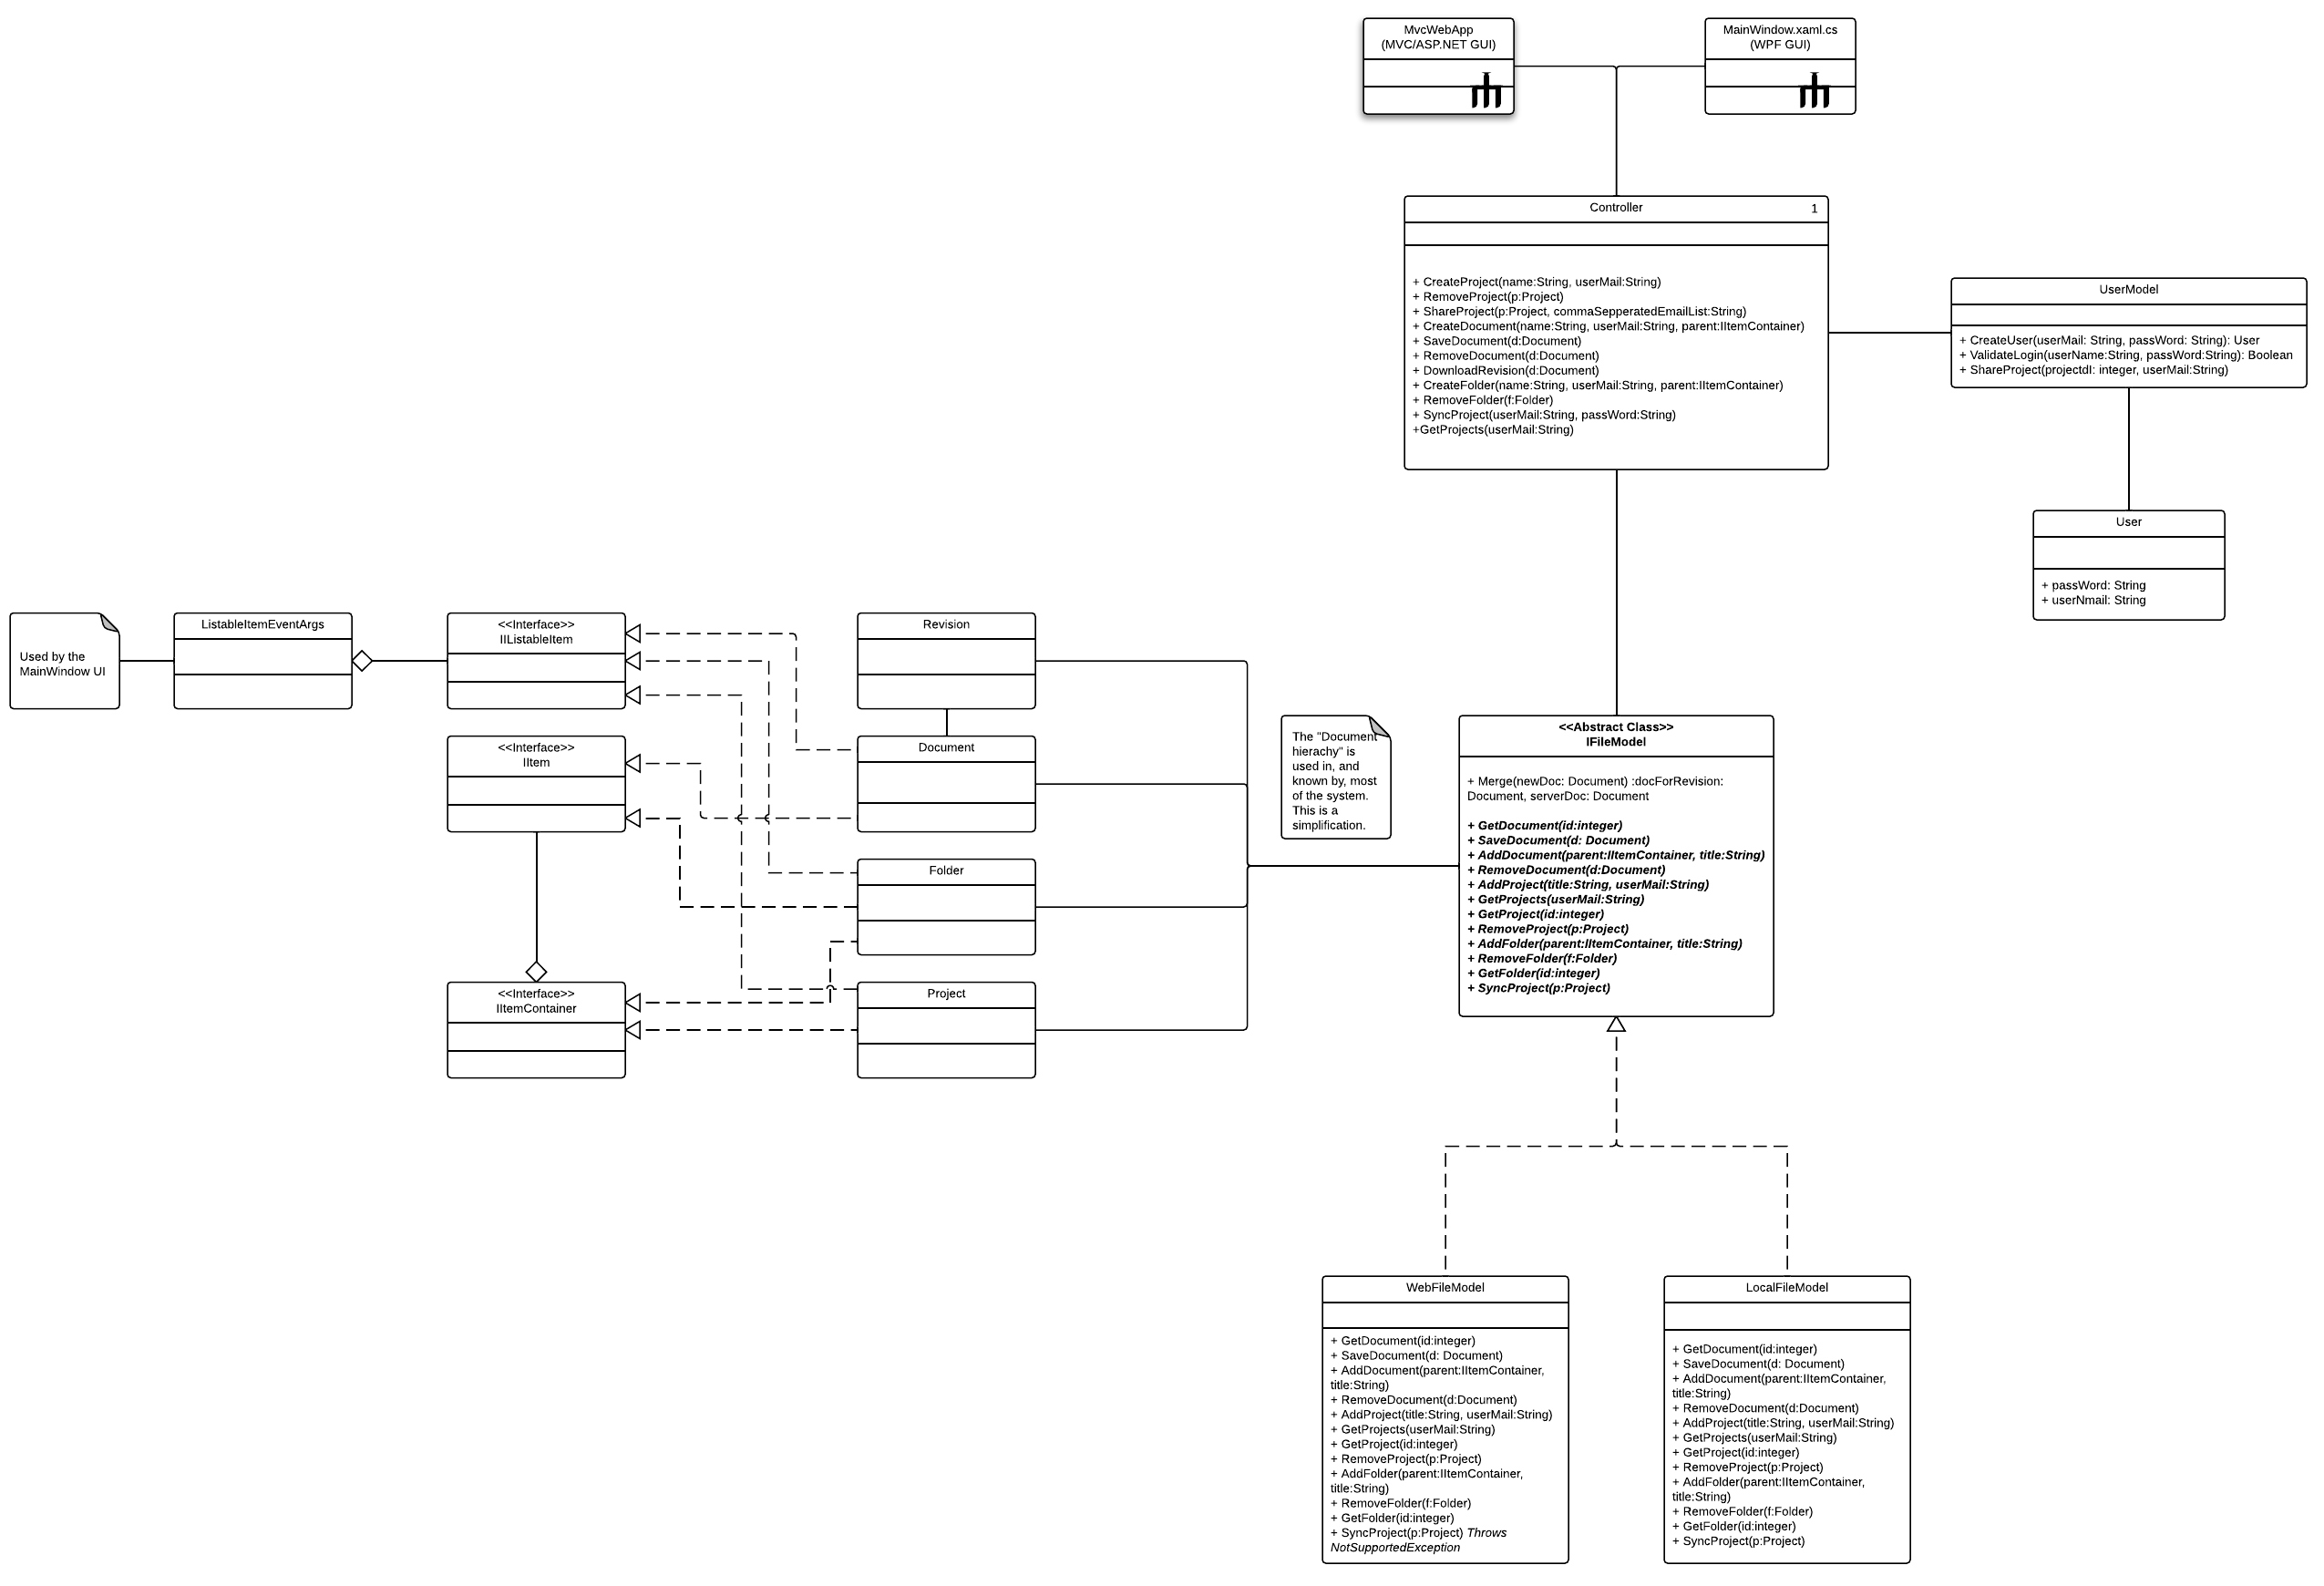
\includegraphics[width=1\textwidth]{Software_design/graphics/mainClassDiagram.png}
        \caption{Overview of the simplified main class diagram for 'Slice of Pie'}
        \label{fig:design-class_diagram} % maybe a link for the web version for full view
    \end{center}
\end{figure}

In (Figure~\ref{fig:design-class_diagram}) the most critical and important classes are shown with their most important attributes and public methods.
None of the two GUIs (MvcWebApp and MainWindow) are shown in the class diagram, but are in two separate class diagrams. This is shown with the rake
symbol on the two classes in the main class diagram.

%Fill in some explanation about the diagram

\subsubsection{The MvcWebApp GUI}

The diagram showing the raked class diagram for the MvcWebApp GUI can be found in the Appendix~\ref{fig:mvcwebapp-diagram}.

We have chosen only to show the controller classes, since they are the most crucial classes for understanding how the Web UI works. The Web UI uses
the ASP.NET MVC3 design pattern. We decided to use MVC since we thought it to be suitable for our needs. 

The 'views' of the MVC3 structure has been omitted. This is done because they do not have any important or interesting functionality except of rendering
the different sites that are available at the Web UI. The methods with a [GET] tag, gets a desired view and the methods with a [POST] tag, posts a HTTP request.

For each method in a controller there is a corresponding view that is rendered when the method is called. However if there are two methods with the same 
name in a controller, where one is a [GET] method and the other is a [POST] method, there is only one view.

The 'models' used are all located in the 'SliceOfPie' project which ensures that consistency between the Web client and the local client.

\subsubsection{The MainWindow GUI}

The diagram showing the raked class diagram for the MainWindow GUI is to be found in the Appendix~\ref{fig:mainwindow-diagram}.
